\documentclass[12pt]{article}
\usepackage[utf8]{inputenc}

\usepackage{amsmath}
\usepackage{bookmark}
\usepackage[a4paper, margin=3.5cm]{geometry}
\usepackage{graphicx} % For inserting images
\usepackage{hyperref} % For hyperlinks
\usepackage{indentfirst}
\usepackage{minted} % For code-highlighting
\usepackage{parskip}

\graphicspath{ {./images/} }
\setlength{\parindent}{15pt} % Set paragraph indentation
\setlength{\parskip}{1em} % Set paragraph space (one line)
\setminted{frame=single, breaklines} % Set codeblock style

\title{Programming Practicum Report:\\Meeting \#3}
\author{\href{https://github.com/avaxar}{R. Ethan Halim}}
\date{September 10th, 2024}

\begin{document}

\maketitle

\section{Quadratic Equation Solver}
The entire source file is hosted on a GitHub repository \href{https://github.com/avaxar/uni-practica-1/tree/main/week_3/01_quadratic}{\textbf{here}}.

\subsection{Explanation}

As the program is to solve the value of $x$ given a quadratic equation, firstly, the program must receive input from the user about the coefficients, which are stored in variables \texttt{a}, \texttt{b}, and \texttt{c}.

\begin{minted}{cpp}
int program(std::istream& cin, std::ostream& cout) {
    double a, b, c;
    cout << "Insert `a`: ";
    cin >> a;
    cout << "Insert `b`: ";
    cin >> b;
    cout << "Insert `c`: ";
    cin >> c;

    ...
}
\end{minted}

\pagebreak
$$ax^2 + bx + c = 0$$
$$\text{discriminant} = D \equiv b^2 - 4ac$$
$$x = \frac{-b \pm \sqrt{D}}{2a}$$

The rest of the program calculates the value of $x$ by the quadratic formula, as detailed above. However, as the program needs to inform the user regarding whether the value(s) of $x$ may be two in amount, solely one, or complex, the intermediate discriminant value is calculated, which is used to check for all of the three cases, as the comments in the code below entail.

\begin{minted}{cpp}
int program(std::istream& cin, std::ostream& cout) {
    ...

    double discriminant = std::pow(b, 2.0) - 4.0 * a * c;
    // If D > 0, then both roots are distinct and real.
    if (discriminant > 0) {
        double x1 = (-b + std::sqrt(discriminant)) / (2.0 * a);
        double x2 = (-b - std::sqrt(discriminant)) / (2.0 * a);

        cout << "\nThe roots are distinct: " << x1 << " and " << x2 << ".\n";
    }
    // If D == 0, then both roots are the same.
    else if (discriminant == 0) {
        double x = (-b + std::sqrt(discriminant)) / (2.0 * a);

        cout << "\nThere is only one real root: " << x << ".\n";
    }
    // If D < 0, then no real roots exist.
    else {
        cout << "\nThe roots are imaginary.\n";
    }

    return 0;
}
\end{minted}

\subsection{Manual Testing}
Below is the compilation and the testing of the source code.
\newline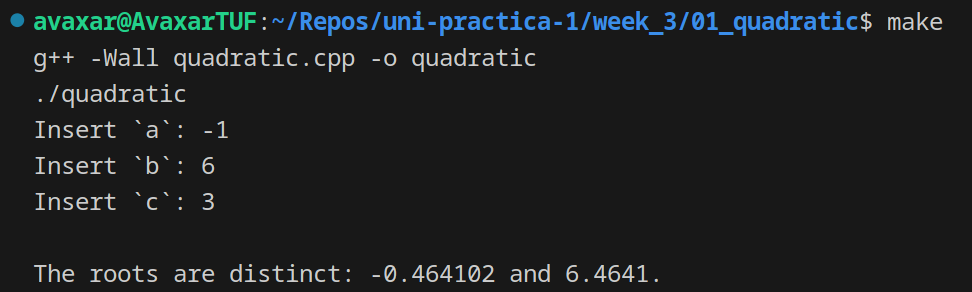
\includegraphics[width=\textwidth]{01_quadratic}

\subsection{Test Cases}

\subsubsection{Tests}
Below is copied directly from the \texttt{tests.txt} file. The first two test cases test for the scenario where there are two distinct real roots; the second two test cases test for the scenario where there is only one single real root; and the third two test cases test for the scenario where the roots are complex.
\inputminted{text}{01_quadratic/tests.txt}

\subsubsection{Execution}
Below are the results of the test cases. No test cases failed.
\newline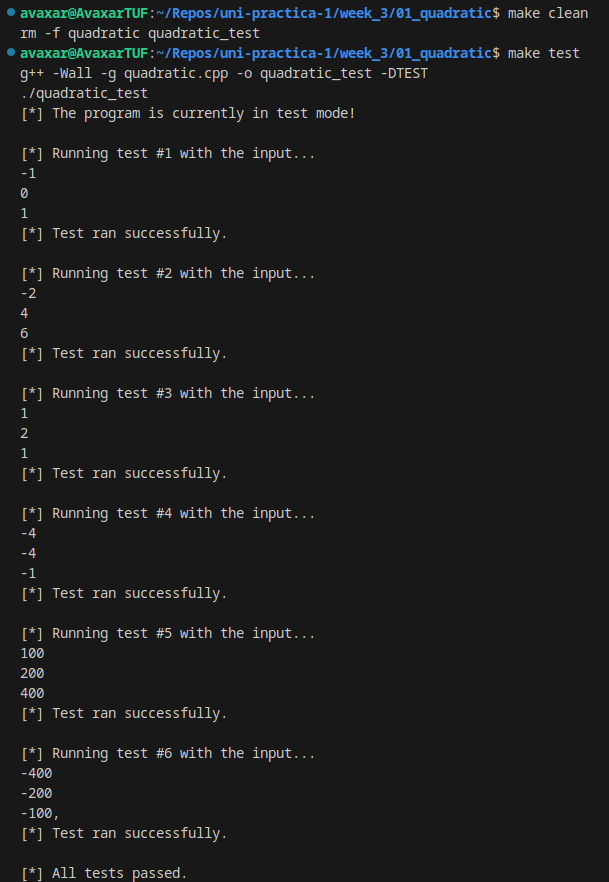
\includegraphics[width=\textwidth]{01_quadratic_test}

\pagebreak
\section{Maximum Number Finder}
The entire source file is hosted on a GitHub repository \href{https://github.com/avaxar/uni-practica-1/tree/main/week_3/02_max_number}{\textbf{here}}.

\subsection{Explanation}

The program is to figure out the maximum value of three given numbers. Firstly, it requests input from the user of those three values, stored as \texttt{n1}, \texttt{n2}, and \texttt{n3}.

\begin{minted}{cpp}
int program(std::istream& cin, std::ostream& cout) {
    double n1, n2, n3;
    cout << "Input the first number: ";
    cin >> n1;
    cout << "Input the second number: ";
    cin >> n2;
    cout << "Input the third number: ";
    cin >> n3;

    ...
}
\end{minted}

It then goes through a series of comparisons between the values to see and reassign the greatest values among them. The variable \texttt{max} is initially assigned to \texttt{n1}, which is then subsequently checked to the value of \texttt{n2} and \texttt{n3} to see which one is greater; figuratively, it is alike to a staging match among each pair of two values. The greatest of the three numbers is then printed out.

\begin{minted}{cpp}
int program(std::istream& cin, std::ostream& cout) {
    ...

    // Generally, using a loop to iterate over all of the remaining elements within an array to check the maximum would be better, in order to reduce code duplication. However, since there are only three elements in total, stored in separate variables, unwound if-statements are used instead.
    double max = n1;
    if (n2 > max) {
        max = n2;
    }
    if (n3 > max) {
        max = n3;
    }

    cout << "\nThe maximum is " << max << ".\n";
    return 0;
}
\end{minted}

\subsection{Manual Testing}
Below is the compilation and the testing of the source code.
\newline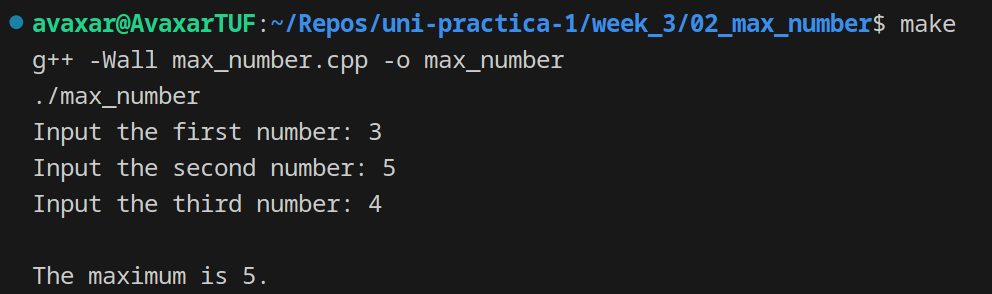
\includegraphics[width=\textwidth]{02_max_number}

\subsection{Test Cases}

\subsubsection{Tests}
Below is copied directly from the \texttt{tests.txt} file.
\inputminted{text}{02_max_number/tests.txt}

\subsubsection{Execution}
Below are the results of the test cases. No test cases failed.
\newline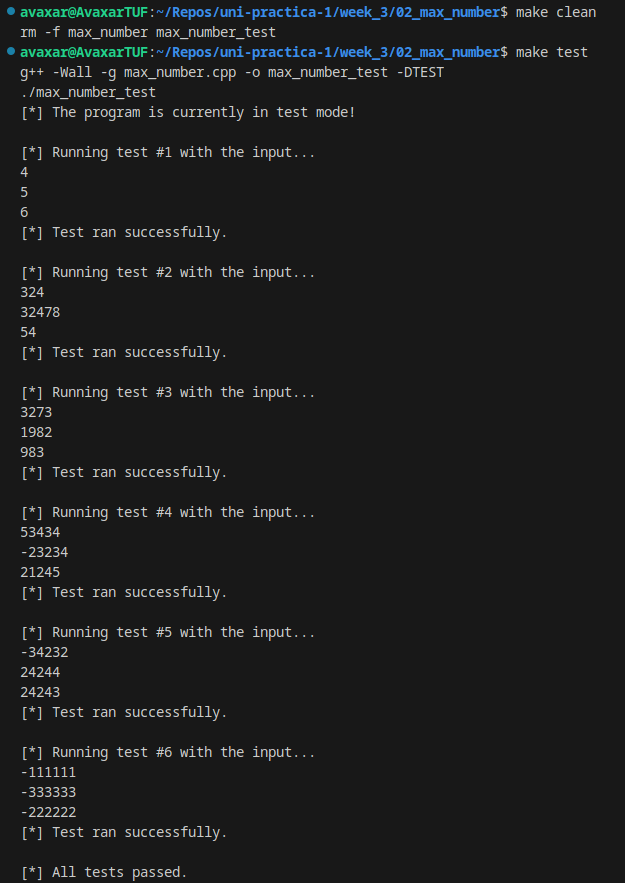
\includegraphics[width=\textwidth]{02_max_number_test}

\pagebreak
\section{Explanation of Branching in C/C++}
In C/C++, like any other conventional programming languages, there are statements which divert the flow of code into separate "branches" depending on the satisfaction of certain conditions. This allows the program to handle multiple possibilities/paths that the user may take, or handle certain conditional cases within any algorithms therein. Akin to a tree, these multiple paths are considered branches; there may be branches within branches; and branches may loop around itself.

\subsection{Goto Statements}

Goto-statements are the barest form of branching, as they enable the programmer to directly jump into certain parts of a function; they perform \textbf{unconditional jumps}. In terms of their usage, a function is to have at least one label, onto which the goto-statement can jump. Goto-statements are the closest that C/C++ offers to Assembly's \texttt{jmp} instruction.

\begin{minted}{cpp}
goto my_label;
a();
my_label:
b();
\end{minted}

In the example above, \texttt{goto my\_label;} will jump onto the part preceding \texttt{b();}. Thus, \texttt{a();} will never get run. In the example below, \texttt{goto my\_label;} will jump onto \texttt{my\_label}, which is placed before the goto-jump. Therefore, this will produce an infinite loop, constantly executing \texttt{a();}.

\begin{minted}{cpp}
my_label:
a();
goto my_label;
\end{minted}

In most cases however, the usage of goto-statements is discouraged, because it is known to be hard to optimize by compilers, which would produce slower binaries. Moreover, there are most likely alternatives which utilize existing constructions provided by the language instead, the usage of which aids readability for the programmers and ease of optimization for the compiler.

\subsection{Conditional Statements}
In this category, statements that perform conditional branching are included. They check for certain satisfied or unsatisfied conditions, and act accordingly as instructed by the programmer. This is the most common form of branching.

\subsubsection{If-Else Statements}
If statements are the most commonly-used forms of branching, as they take an expression which either returns \texttt{true} or \texttt{false}, both of which determine whether the enclosed code within the statement is to be executed or not. Below is the boilerplate for an if statement.

\begin{minted}{cpp}
if (condition) {
    code();
}

rest();
\end{minted}

If the given expression (represented by the variable \texttt{condition}) returns \texttt{true}, then it will execute the code enclosed within the brackets after it; in this case, it will call the function named \texttt{code}. Regardless of the truth value of \texttt{condition} (i.e. whether the if-statement is satisfied), the code following the conclusion of the if-statement will be run, that is the function named \texttt{rest} in this case, which resumes back onto the main branch of the code.

In order to handle both cases where \texttt{condition} returns either \texttt{true} or \texttt{false}, with the focus being on the latter, an else-statement may be put following the if-statement. This splits the main branch into two subbranches that the code execution may take.

\begin{minted}{cpp}
if (condition) {
    planA();
}
else {
    planB();
}
\end{minted}

In the code above, if the \texttt{condition} is satisfied, then \texttt{planA} will be run; if it isn't, then \texttt{planB} will be run instead. If \texttt{planA} and \texttt{planB} were return statements within a value-returning function, then the said function would be mathematically similar to the formula below.

$$f(...) = \begin{cases}
    a() & \text{if } condition \\
    b() & \text{if } \neg condition
\end{cases}$$

Additionally, multiple if-statements can be chained together to check for and handle multiple conditions, as written below for instance.

\begin{minted}{cpp}
if (conditionA) {
    planA();
}
else if (conditionB) {
    planB();
}
else if (conditionC) {
    planC();
}
else {
    planD();
}
\end{minted}

However, if the conditions above involved the equality of the same expression with different integers or characters, a switch-statement would be more appropriate for such use case.

\subsubsection{Switch Statements}

Switch-statements are similar to a chain of if-statements which check for multiple conditions when it comes to checking for and handling multiple equality conditions between a given expression and the provided cases. Thus, this snippet of code involving the switch-statement below ...

\begin{minted}{cpp}
switch (x) {
    case 1:
        planA();
        break;
       case 2:
        planB()
        break;
       case 3:
        planC();
        break;
       default:
        planD();
}
\end{minted}

... is equivalent to the chain of if-statements below ...

\begin{minted}{cpp}
if (x == 1) {
    planA();
}
else if (x == 2) {
    planB();
}
else if (x == 3) {
    planC();
}
else {
    planD();
}
\end{minted}

... and is similar to the mathematical formula below.

$$f(...) = \begin{cases}
    a() & \text{if } x = 1 \\
    b() & \text{if } x = 2 \\
    c() & \text{if } x = 3 \\
    d() & \text{if neither}
\end{cases}$$

In order to add more cases, one can add more \texttt{case} labels followed by the integer or character constant they please and a colon. \texttt{break;} statements following the conclusion of each case are necessary as to quit the switch-statement upon case-completion. Otherwise, code execution would run into other cases, which may not be desirable. This code snippet below ...

\begin{minted}{cpp}
switch (x) {
    case 1:
        planA();
    case 2:
        planB()
}
\end{minted}

... would be equivalent to the code below, as the execution from \linebreak \texttt{planA();} would spill over downwards, with nothing halting it preceding the \texttt{case 2:} label.

\begin{minted}{cpp}
if (x == 1) {
    planA();
    planB();
}
else if (x == 2) {
    planB();
}
\end{minted}

The reason why one may need to prefer switch-statements over if statement is because switch-statement offer more performance, as the compiler is able to recognize and perform optimizations in a way which does not involve having to check for every single given condition, as how an if-statement would be handled. The resulted binary would receive gains in performance.

\subsection{Looping}
Loops are parts of code that are executed repeatedly (multiple times) in a sequential manner, given a condition which defines how many times the given code should be run, or until when the looping should be stopped. On each iteration, the code may receive different inputs or interact with the changes made by its previous iterations.

\subsubsection{While Loops}
A while-loop is the most basic form of loops. Given the satisfaction of a condition, the code within will always be run over and over until the said condition is no longer satisfied; from which, code execution will resume out of the loop.

\begin{minted}{cpp}
while (condition) {
    code();

    // Upon the end of the code, `condition` is reevaluated of its truth value, in order to determine whether the loop should continue.
}
\end{minted}

In the example above, the value of \texttt{condition} will be determined of its truth value (either \texttt{true} or \texttt{false}). If it is \texttt{true}, then \texttt{code} will get executed. Upon completion, the \texttt{condition} will be checked again and the cycle repeats. If \texttt{condition} were set to always be \texttt{true}, then it would be an infinite loop with no foreseeable end.

In order to illustrate how while-loops work beneath the abstractions of the language, if the snippet were rewritten using \texttt{goto} and \texttt{if}, it would look as follows. \texttt{start:} and \texttt{end} are jump labels representing the start and end of the loop respectively.

\begin{minted}{cpp}
start:
// If `condition` is no longer satisfied, it will end the loop.
if (!condition) {
    goto end;
}

// What is contained in the loop starts here.
code();

goto start; // Loops back for condition-rechecking
end:
\end{minted}

Midway inside a while-statement, loop-halting and iteration-skipping can be controlled directly using \texttt{break;} and \texttt{continue;}. \texttt{break;} stops and ends the loop immediately regardless of the value of \texttt{condition}. \texttt{continue;} stops and ends the current iteration of the loop. These two statements are available in all of the loop types in the language and apply similarly.

\begin{minted}{cpp}
while (condition1) {
    if (condition2) {
        break;       }
    else {
        continue;
    }
}
\end{minted}

The boilerplate above is equivalent to the code snippet below which illustrates the destination of the jumps made by the two statements using goto-statements.

\begin{minted}{cpp}
while (condition1) {
    if (condition2) {
        goto loop_end; // formerly `break;`
    }
    else {
        goto iteration_end; // formerly `continue;`
    }

iteration_end:
    // From here, `condition1` will be reevaluated of its truth value, in order to determine whether the loop should continue.
}
loop_end:
\end{minted}

\subsubsection{Do-While Loops}
Do-while-loops are similar to while-loops, however the code within is executed on the first iteration regardless of the given condition. They have the syntax as follows ...

\begin{minted}{cpp}
do {
    code();
} while (condition);
\end{minted}

... which is equivalent to the code snippet below using a regular while-loop.

\begin{minted}{cpp}
code();
while (condition) {
    code();
}
\end{minted}

\subsubsection{For Loops}
For-loops are loops which act as "condensed" while-loops. They accept an initializing statement, a condition expression, and a post-iteration statement. Their syntax is as follows ...

\begin{minted}{cpp}
for (INITIAL; condition; POST) {
    code();
}
\end{minted}

... which is equivalent to the code snippet below using a regular while-loop.

\begin{minted}{cpp}
INITIAL;
while (condition) {
    code();
    POST;
}
\end{minted}

Typically, for-loops are used to iterate over a range of numbers. For that reason, the initializing statement tends to be a variable declaration which declares and defines the iterating variable (a.k.a \textit{iterator}), commonly named \texttt{i}. The condition after it defines whether the variable is part of the given range. The post-iteration statement increments or decrements the iterator, in order to loop onto the next number in the range. Below is a code example which iterates and prints numbers from 1 to 5.

\begin{minted}{cpp}
for (int i = 1; i <= 5; i++) {
    std::cout << i << '\n';
}
\end{minted}

The iterator starts out at \texttt{1} and gets printed to the terminal. The post-iteration statement increments the iterator by 1, and thus the iterator becomes \texttt{2}. This repeats until the end of the iteration where the iterator is \texttt{5}, whereby the incrementation of the iterator invalidates the loop condition (i.e. \texttt{i <= 5} is no longer satisfied), thereby stopping it before \texttt{6} would be printed.

\subsubsection{For-Each Loops}
For-each-loops (alternatively called \textit{ranged-for-loops}) are a loop type which was added in C++11, and is not present in C. They are syntactic sugar which aids in iterating over the elements of a collection (typically of a container type implemented by the C++ STL [standard template library]). For instance, when used with a \texttt{std::vector} instance, it will loop over each element starting with the lowest index (from 0). The boilerplate in doing so is as follows.

\begin{minted}{cpp}
std::vector<int> vec = {9, 7, 5, 3, 1};
for (int e : vec) {
    // Prints "9 7 5 3 1" in sequence
    std::cout << e << ' ';
}
\end{minted}

In this case, the "iterator [variable]" refers to the variable which is declared to funnel every element of the vector (that is, \texttt{e}). In the context of iterating over a \texttt{std::vector}, the example usage above offers better readability and general beauty than the alternate implementation below, which solely uses a regular for-loop.

\begin{minted}{cpp}
std::vector<int> vec = {9, 7, 5, 3, 1};
for (int i = 0; i < vec.size(); i++) {
    int e = vec[i];

    // Prints "9 7 5 3 1" in sequence
    std::cout << e << ' ';
}
\end{minted}

\subsection{Function Calling}
\begin{minted}{cpp}
return_type function([argument_type1 argument1, [argument_type2 argument2, ...]]) {
    code();
}
\end{minted}

Functions are pieces of code which may call other functions or themselves, in a way that lets them to be reusable. They enclose technicalities and pack them into more abstract "tools", such that the end-programmer may use them imperatively in the main code without worrying how it works below the hood or rewriting them over and over on demand. They work similarly to functions in mathematics, where they can accept arguments and return a value. The following mathematical function which does a dot product from its given arguments ...

$$dot(ax, ay, bx, by) = ax * bx + ay * by$$

... is equivalent to the code below, where the type of the numeric arguments and return value is expected to be a real number, using \texttt{double}.

\begin{minted}{cpp}
double dot(double ax, double ay, double bx, double by) {
    return ax * bx + ay * by;
}
\end{minted}

However, functions in programming can do much more than what they can do in math. They do not necessarily have to include a return value (for such case, the return type would be \texttt{void}). They enclose programming statements/instructions; they are more akin to procedures. In fact, the \texttt{main} function is itself a function, where statements live and are executed. Function calling acts more similarly to code-substitution, as illustrated below.

\begin{minted}{cpp}
void func() {
    std::cout << "Hello, world!\n";
    std::cout << "I am `func`.\n";
}

int main() {
    func()
}
\end{minted}

\begin{minted}{cpp}
int main() {
    // Calling `func` is similar to writing directly below.
    std::cout << "Hello, world!\n";
    std::cout << "I am `func`.\n";
}
\end{minted}

In practical use, they help uphold the DRY ("do not repeat yourself") rule, as repetitive similar blocks of code cluttered around a codebase can be refactored in a way such that the said code is only written once. As they can call themselves, \textit{recursion} can be utilized to make code more compact when dealing with tree-related data structures or certain algorithms, such as generating the Fibonacci sequence.

\begin{minted}{cpp}
int fib(int n) {
    // Base cases, where the recursion will hit an end
    if (n == 0) {
        return 0;
    }
    if (n == 1) {
        return 1;
    }

    // Calls itself, making two branches
    return fib(n - 1) + fib(n - 2);
}
\end{minted}

\pagebreak
If \texttt{fib} is called with its argument as \texttt{6} by \texttt{fib(6)}, then multiple branching recursions will entail, as illustrated in the tree diagram below, courtesy of \href{https://willrosenbaum.com/assets/img/recursive-fibonacci/tree.png}{\textbf{this resource}}.
\newline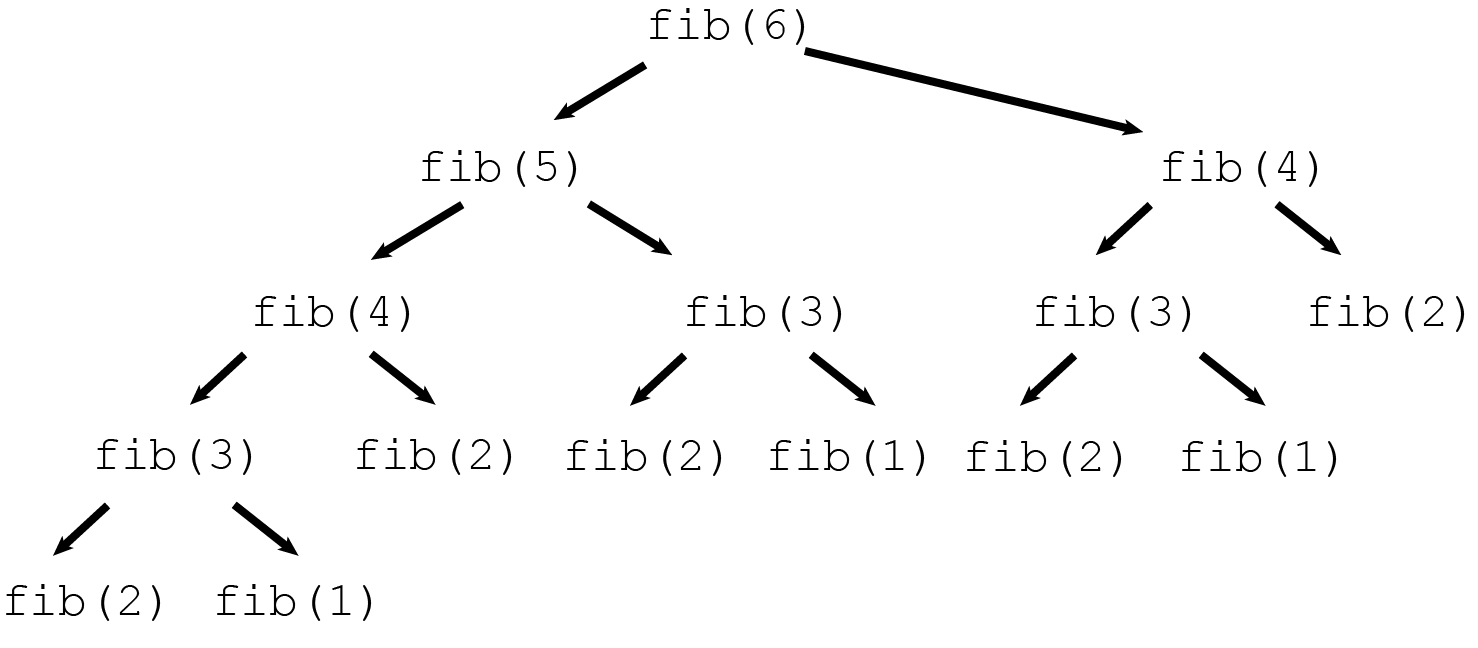
\includegraphics[width=\textwidth]{fibonacci}

\subsection{Exceptions}
Exceptions are sudden jumps in code, possibly across functions, made due to unexpected errors that are to be handled. They are a feature exclusive to C++ and does not exist in C. While they are not conventional branchings, they still cause diversion in control flow upon the throwing of an exception. The said throwing is a programmer-written indication that something went wrong within the code, and the code above must handle it, in order to not let the program crash.

\subsubsection{Throw Expressions}
Take an example where a programmer is writing a function which may fail upon certain circumstances. They would need to be able to indicate and panic out of the function for the end-programmer, in order to let the code that is using the function know. Throw expressions in C++ lets the programmer throw an object, conventionally an instance of the base class \texttt{std::exception}, which entails the underlying error. Below is an example function which encapsulates division with a check to detect for any zero-divisions.

\begin{minted}{cpp}
throw EXPRESSION;
\end{minted}

\begin{minted}{cpp}
int divide(int a, int b) {
    if (b == 0) {
        throw std::runtime_error("Zero division occurred");
    }

    return a / b;
}
\end{minted}

If \texttt{divide} were to be called with the argument \texttt{b} set as zero, an exception object---an \texttt{std::runtime\_error} instance (a subclass inheriting the STL base class \texttt{std::exception}), which contains the given error message (\texttt{"Zero division occurred"}), would be thrown and the function would immediately be exited along with any other functions that had called it until the exception is caught to be handled, the process of which is explained in the next section.

\subsubsection{Catching Exceptions}
Following from before, after the exception has been thrown, it needs to be caught; otherwise, if the exception unwound upwards reaching the \texttt{main} function, the program would crash. In order to catch exceptions, a try-block must enclose the potential exception-throwing code and a catch-block must be present, which entails the code to deal with the thrown exception object and act appropriately upon the faulty case.

\begin{minted}{cpp}
try {
    code();
}
catch (VARIABLE_DECLARATION) {
    handler();
}
\end{minted}

Resuming from the \texttt{divide} function implemented before, in order to catch for any errors given out by the function, the function call must be enclosed inside a try-block. The \texttt{VARIABLE\_DECLARATION} following the \texttt{catch} keyword holds a reference to the thrown exception object. In the example below, although what was thrown is an \texttt{std::runtime\_error} object, since it inherits \texttt{std::exception} as its base class, polymorphism lets the object be cast up, exposing the \texttt{.what()} method to yield its error message.

\begin{minted}{cpp}
int result;
try {
    result = divide(1, 0);
}
catch (const std::exception& exc) {
    std::cerr << "Exception was thrown, saying: " << exc.what() << '\n';
}
\end{minted}

If the code in the catch-block cannot proceed with resolving the issue, then the exception can be rethrown, so that the exception may be passed upwards to the calling function until it is again handled or the program crashes.

\begin{minted}{cpp}
catch (const std::exception& exc) {
    // The block cannot handle the exception, thus
    // the exception is rethrown.
    throw;
}
\end{minted}

\end{document}
